\documentclass[xcolor={x11names}]{beamer}
\usetheme{Madrid}

\usepackage{amssymb}
\usepackage{mdframed}
\usepackage{ulem}
\usepackage[utf8]{inputenc}
\usepackage{mathtools}
\usepackage{multicol}
%\usepackage[x11names]{xcolor}
\usefonttheme{professionalfonts}


% Subfigures
\usepackage{caption}
\usepackage{subcaption}


% License
\usepackage[
    type={CC},
    modifier={by-nc-sa},
    version={4.0},
    imagewidth=4pt
]{doclicense}




% Change base colour beamer@blendedblue (originally RGB: 0.2,0.2,0.7)
\colorlet{beamer@blendedblue}{DarkSeaGreen4}







%% MATH commands
\DeclareMathOperator{\Var}{Var}


%% THEOREMS
%\newtheorem{theorem}{Theorem}
\newtheorem{thm}{Teorema}[section] % the main one
% Definición
%\theoremstyle{definition}
\newtheorem{definicion}{Definición}[section]
\newtheorem{lema}{Lema}[section]



%% PFGplots %%
\usepackage{pgfplots}

%% Exponential distribution
\pgfmathdeclarefunction{exponential}{1}{%
  \pgfmathparse{(#1)*exp(-#1*x)}%
}
\pgfmathdeclarefunction{exponentialcdf}{1}{%
  \pgfmathparse{1-exp(-#1*x)}%
}

%% Poisson distribution
\pgfmathdeclarefunction{poiss}{1}{%
  \pgfmathparse{(#1^x)*exp(-#1)/(x!)}%
}

%% Normal distribution (#1=mu, #2=sigma)
% John D. Cook approx. https://tex.stackexchange.com/a/124629
\pgfmathdeclarefunction{normalcdf}{2}{%
  \pgfmathparse{1/(1 + exp(-0.07056*((x-#1)/#2)^3 - 1.5976*(x-#1)/#2))}%
}




\newcommand{\red}[1]{{\color{red}#1}}
\newcommand{\blue}[1]{{\color{blue}#1}}

%%%%%%%%%%
%% TIKZ %%
%%%%%%%%%%
\usepackage{tikz}
\usepackage{animate}
\usetikzlibrary{positioning}
\usetikzlibrary{shapes,arrows, positioning, calc}
\usetikzlibrary{overlay-beamer-styles}
\usetikzlibrary{chains,shapes.multipart}
\usetikzlibrary{scopes}
\usetikzlibrary{automata}
\usetikzlibrary{positioning}  %                 ...positioning nodes
\usetikzlibrary{arrows}       %                 ...customizing arrows
\usetikzlibrary{intersections}


%%%%%%%%%
%% PGF %%
%%%%%%%%%
\usepgfplotslibrary{fillbetween}


%%% Insert section name before the section %%%
\AtBeginSection[]{
  \begin{frame}
  \vfill
  \centering
  \begin{beamercolorbox}[sep=8pt,center,shadow=true,rounded=true]{title}
    \usebeamerfont{title}\insertsectionhead\par%
  \end{beamercolorbox}
  \vfill
  \end{frame}
}



\title[Tema 5]{Tema 5: Servicios y
Calidad de Servicio\\Cálculo de Redes}
%% \subtitle{Redes y Servicios de Telecomunicaciones (RSTC)\\
%% Grado en Ingeniería de Tecnologías y Servicios de Telecomunicación}
%\author{M. Saiful Bari\inst{1} \and Mr X\inst{2}}

\titlegraphic{%

\includegraphics[height=2cm]{figs/RSTC-grande.png}\\%
\doclicenseIcon {\tiny \hspace{1em}\doclicenseText}\\%
\href{https://github.com/MartinPJorge/RSTC-netcal-slides}{
\includegraphics[height=1cm]{figs/github-logo.png}}%
}

\author{\textcolor{white}{RSTC curso 2024-2025}}
%\author{Jorge Martín Pérez\inst{1}}
%\institute{
%    \inst{1}
%    Departamento de Ingeniería Telemática, Universidad Politécnica de Madrid
%}

\date{\today}







%%%%%%%%%%%%%%%%%%%%
%%% SLIDES START %%%
%%%%%%%%%%%%%%%%%%%%
\begin{document}


%%% TITLE %%%
\frame{\titlepage }


\begin{frame}[allowframebreaks]{Contenido}
    \tableofcontents
\end{frame}




\section{Introducción}
\begin{frame}{\secname}
    El cálculo de redes modela flujos
    \begin{itemize}
        \item electricidad
        \item fluidos
        \item \textbf{tráfico en internet}
    \end{itemize}

    \vfill
    Nos sirve para modelar:
    \begin{itemize}
        \item conformado de tráfico
        \item políticas de tráfico
        \item averiguar métricas de
            lantencia y tamaño en cola
    \end{itemize}
\end{frame}



\section{Álgebra min-plus}
\begin{frame}{\secname}
    \begin{definicion}[Álgebra min-plus]
        Es un diodo\footnote{Un tipo de
        estructura algebraica.}
        definido en
        $(\mathbb{R}\cup \{+\infty\},
        \land, +)$, donde:
        \begin{itemize}
            \item $\land$ es el operador
                $\min$
            \item $+$ es la suma
        \end{itemize}
    \end{definicion}

    \vfill

    \emph{Ejemplo}:

    la operación
    \begin{equation*}
        (1+2)\cdot 3 = 9
    \end{equation*}
    se ``traduce'' en:
    \begin{equation*}
        (1\land2)+ 3 = 4
    \end{equation*}
\end{frame}



\begin{frame}{\secname}
    \begin{definicion}[Familia de funciónes crecientes]
        Sea $\mathcal{F}$ el conjunto 
        de funciones crecientes, decimos
        que $f\in\mathcal{F}$ es una función
        creciente definida en
        $f:\mathbb{R}^+\mapsto\mathbb{R}^+$
        si y sólo si cumple:
        \begin{equation}
            f(s)\geq f(t), \forall s\geq t
        \end{equation}
        y además
        $f(t)=0,\forall t<0$.
    \end{definicion}

    \vfill

    \emph{Ejemplo}: la función ``rate-latency''
    $\beta_{R,T}(t)=R[t-T]^+$



    \begin{figure}[h]
        \centering
        \begin{tikzpicture}[
  declare function={
    ratelatency(\R,\T,\x)= (\x<=\T) * 0   +
    (\x>\T) * (\R*(\x-\T));
    }
]
\begin{axis}[
    x=1cm,
    y=1cm,
    domain=0:5,
    ymin=0,
    xmin=0,
    axis x line=middle,
    axis y line=middle,
     xlabel style={
            anchor=west,
            at={(ticklabel* cs:1.0)},
            xshift=5pt
        },
        xlabel=$t$,
    ]
    \addplot[DodgerBlue3,ultra thick,smooth]
        {ratelatency(0.5,1,x)};
\end{axis}
\end{tikzpicture}

    \end{figure}

\end{frame}


\subsection{Convolución}
\begin{frame}{\secname: \subsecname}
    \begin{definicion}[Convolución min-plus]
        La convolución
        min-plus
        $\otimes$ de dos
        funciones crecientes
        $f,g\in\mathcal{F}$
        se define como
        \begin{equation}
            (f\otimes g)(t)
            =\inf_{0\leq s\leq t}
            \{f(t-s)+g(s)\}
        \end{equation}
    \end{definicion}

    \vfill

    \emph{Nota}: equivalente
    a la convolución
    ``clásica'':
    \begin{equation*}
        (f\ast g)(t)
        =\int_0^t
        f(t-s)g(s)\ ds
    \end{equation*}
\end{frame}






\begin{frame}{\secname: \subsecname}
    Si $f(0)=g(0)=0$ se puede
    calcular
    comenzando a dibujar
    cada función sobre
    todo punto de la
    otra y tomando
    el mínimo.
    \vfill
    \begin{figure}[h]
        \centering
        \begin{tikzpicture}[
  declare function={
    ratelatency(\R,\T,\x)= (\x<=\T) * 0   +
    (\x>\T) * (\R*(\x-\T));
    }
]
\begin{axis}[
    x=1cm,
    y=1cm,
    domain=0:5,
    ymin=0,
    xmin=0,
    axis x line=middle,
    axis y line=middle,
     xlabel style={
            anchor=west,
            at={(ticklabel* cs:1.0)},
            xshift=5pt
        },
    xlabel=$t$,
    legend pos=outer north east
    ]
    \addplot[DodgerBlue3,ultra thick,smooth]
        {ratelatency(0.75,2,x)};
    \addplot[Firebrick3,ultra thick,smooth]
        {0.4*x};

    \addplot[Gold3,ultra thick,smooth]
        {ratelatency(0.4,2,x)};

    \foreach \t in {.5,1.5,2.5,3.5,4.5}  {
        
        \addplot[DodgerBlue2,smooth,domain=\t:5]
        {ratelatency(0.75,2,x-\t)+0.4*\t};
    }


    \legend{
    $g(t)$,
        $f(t)$,
    $(f\otimes g)(t)$};

\end{axis}
\end{tikzpicture}

    \end{figure}


    \vfill

    En este ejemplo:
    $f(t)=rt,
    g(t)=\beta_{R,T}(t)$
    con $R>r>0$.
\end{frame}



\begin{frame}{\secname: \subsecname}
    Calculemos la
    convolución min-plus
    de manera analítica:
    \begin{equation*}
        (f\otimes g)(t)
        =\inf_{0\leq s \leq t}
        \{f(t-s)+g(s)\}
        =\inf_{0\leq s \leq t}
        \{r(t-s)+R[s-T]^+\}
    \end{equation*}

    \pause

    \emph{Con $T\geq t$}:
    \begin{equation*}
        (f\otimes g)(t)
        =\inf_{0\leq s \leq t}
        \{r(t-s)+0\}=0
    \end{equation*}

    \pause

    \emph{Con $T< t$}
    dividimos en dos casos y
    tomamos el menor
        \pause
    \begin{enumerate}
        \item $0\leq s\leq T$:
        \begin{equation*}
            (f\otimes g)(t)
        =\inf_{0\leq s \leq T < t}
        \{r(t-s)+0\}=r(t-T)
        \end{equation*}
        \pause
    \item $T<s$:
        \begin{equation*}
            (f\otimes g)(t)
        =\inf_{T< s \leq t}
        \{r(t-s)+R(s-T)\}
        =r(t-T)
        \end{equation*}
    \end{enumerate}

    \pause
    El resultado es:
    \begin{mdframed}[rightmargin=20em]
        $(f\otimes g)(t)
        =r[t-T]^+$.
    \end{mdframed}

\end{frame}



%%% \begin{frame}{\secname: EJercicio}
%%% Calcule la convolución min-plus
%%% de las función rate-burst
%%% $\gamma_{r,b}(t)=rt+b$
%%% y la función rate-latency
%%% $\beta_{R,T}(t)=R[t-T]^+$.
%%% Obtenga la solución de manera analítica.
%%% 
%%% 
%%% Tenemos:
%%% \begin{equation*}
%%% (\gamma_{r,b}\otimes \beta_{R,T})(t)
%%% =\inf_{0\leq s \leq t}\{r(t-s)+b+R[s-T]^+\}
%%% \end{equation*}
%%% Con $t\leq T$ tenemos
%%% \begin{equation*}
%%% (\gamma_{r,b}\otimes \beta_{R,T})(t)
%%% =\inf_{0\leq s \leq t}\{r(t-s)+b+0\}=b
%%% \end{equation*}
%%% y con $t>T$ tenemos dos casos.
%%% El primero es $s<T<t$:
%%% \begin{equation*}
%%% (\gamma_{r,b}\otimes \beta_{R,T})(t)
%%% =\inf_{0\leq s \leq T}\{r(t-s)+b+0\}=r(t-T)+b
%%% \end{equation*}
%%% y el segundo es $T<s\leq t$
%%% \begin{equation*}
%%% (\gamma_{r,b}\otimes \beta_{R,T})(t)
%%% =\inf_{T< s \leq t}\{r(t-s)+b+R(s-T)\}=r(t-T)+b
%%% \end{equation*}
%%% 
%%% Por tanto la solución es
%%% \begin{equation*}
%%% (\gamma_{r,b}\otimes \beta_{R,T})(t)
%%% =r[t-T]^++b
%%% \end{equation*}
%%% 
%%% \end{frame}




\begin{frame}{\secname: \subsecname}
    La convolución min-plus
    está dotada de las
    siguientes
    propiedades en $\mathcal{F}$:
    \begin{itemize}
        \item \textbf{Cierre}:
            $\forall f,g\in\mathcal{F},\quad f\otimes g\in\mathcal{F}$
        \pause
        \item \textbf{Asociativa}:
            $\forall f,g,h\in\mathcal{F},
            \quad 
            (f\otimes g)
            \otimes h
            =
            f\otimes
            (g\otimes h)$
        \pause
        \item \textbf{Conmutativa}:
            $\forall
            f,g\in\mathcal{F},
            \quad
            f\otimes g=
            g\otimes f$
        \pause
    \item \textbf{Elemento neutro\footnote{$\delta_0(t)=+\infty$ con $t>0$ y 0 con $t\leq0$}}:
            $\exists\delta_0\in\mathcal{F}: \forall f\in\mathcal{F},
            f\otimes\delta_0=f$
        \pause
    \item \textbf{Distrib. con $\land$}:
        $f,g,h\in\mathcal{F},
        \quad
        (f\land g)\otimes h
        = 
        (f\otimes h)
        \land
        (g\otimes h)$
    \pause
    \item \textbf{Suma constante}:
        $\forall f,g\in\mathcal{F},K\in\mathbb{R}^+,
        \quad
        (f+K)\otimes g
        =(f\otimes g) + K$

    \pause
    \item \textbf{Isotonicidad}:
        $\forall f,g,f',g'\in\mathcal{F},\quad
        f\leq f',g\leq g'
        \implies
        f\otimes f'
        \leq
        g\otimes g'$
    \end{itemize}
\end{frame}


\subsection{Deconvolución}
\begin{frame}{\secname: \subsecname}
    \begin{definicion}[Deconvolución min-plus]
        La deconvolución\footnote{No
        esta definida si
        $\exists t: f(t)=+\infty
        $ o $g(t)=+\infty$.}
        min-plus
        $\oslash$ de dos
        funciones crecientes
        $f,g\in\mathcal{F}$
        se define como
        \begin{equation}
            (f\oslash g)(t)
            =\sup_{u\geq0}
            \{f(t+u)-g(u)\}
        \end{equation}
    \end{definicion}

    \vfill

    \emph{Truco}:
    es como la convolución
    min-plus pero sustituyendo
    los $+$ por $-$.
\end{frame}




\begin{frame}{\secname: \subsecname}
    La deconvolución de
    $f(t)=\gamma_{r,b}(t)
    =rt+b$
    y $g(t)=\beta_{R,T}(t)$
    es\footnote{con $R>r$}
    \vfill
    \begin{figure}[h]
        \centering
        \begin{tikzpicture}[
  declare function={
    ratelatency(\R,\T,\x)= (\x<=\T) * 0   +
    (\x>\T) * (\R*(\x-\T));
    }
]
\begin{axis}[
    x=1cm,
    y=1cm,
    domain=-3:5,
    ymin=0,
    xmin=-3,
    axis x line=middle,
    axis y line=middle,
     xlabel style={
            anchor=west,
            at={(ticklabel* cs:1.0)},
            xshift=5pt
        },
    xlabel=$t$,
    legend pos=outer north east
    ]
    \addplot[DodgerBlue3,ultra thick,smooth]
        {ratelatency(0.9,1.3,x)};
    \addplot[Firebrick3,ultra thick,samples=1000]
        {(x>0)*(0.3*\x+1.1) + (x<0)*0};

    \addplot[Gold3,ultra thick,smooth,samples=1000]
        {(x>=-1.3)*(0.3*(\x+1.3)+1.1)+and(x>-2.6,x<-1.3)*(1.1+0.9*\x+0.9*1.3)};



    \legend{
    $g(t)$,
        $f(t)$,
    $(f\oslash g)(t)$};

   \node (burstop) at (axis cs:0.1,1.2){};
   \node (burstbottom) at (axis cs:0.1,-.1){};
   \draw[|-|](burstop)--(burstbottom)
       node[midway,right]
       {$b$};

   \draw[|-|, gray]
       (axis cs:.15,.2)
       --
       (axis cs:1.3,.2)
       node[pos=.9,above]
       {$T$};

   \draw[|-|, gray]
       (axis cs:-.05,.2)
       --
       (axis cs:-1.3,.2)
       node[midway,above]
       {$T$};


\end{axis}
\end{tikzpicture}

    \end{figure}


    \vfill

    \emph{Nota}: nótese
    que $(f\oslash g)(t)
    \notin \mathcal{F}$
    porque no es cero para
    $t<0$.
\end{frame}



\begin{frame}{\secname: \subsecname}
    Calculemos analíticamente
    la deconvolución:
    \begin{equation*}
        (\gamma_{r,b}
        \oslash
        \beta_{R,T})(t)
        =\sup_{u \geq0}
        \{
        \gamma_{r,b}(t+u)
        - \beta_{R,T}(u)
        \}
    \end{equation*}
    recordando que
    $\beta_{R,T}(u)=0,
    t\leq T$ dividimos en dos
    casos
    \pause
    \begin{equation*}
        (\gamma_{r,b}
        \oslash
        \beta_{R,T})(t)
        =\sup_{T>u \geq0}
        \{
        \gamma_{r,b}(t+u)
        \}
        \lor
        \sup_{u>T}
        \{
        \gamma_{r,b}(t+u)
        -
        \beta_{R,T}(u)
        \}
    \end{equation*}
    \pause
    en el primer caso
    $u$ llega a $T$
    y
    $\gamma_{r,b}(t+u)=0,
    t\leq-T$.
    Por tanto tenemos dos casos
    \begin{enumerate}
        \item $t\leq-T$:
    \begin{multline*}
        % (\gamma_{r,b}
        % \oslash
        % \beta_{R,T})(t)
        % =
        0
        \lor
        \sup_{-t\geq u>T}
        \{
        \gamma_{r,b}(t+u)
        -
        \beta_{R,T}(u)
        \}
        \lor
        \sup_{u>-t}
        \{
        \gamma_{r,b}(t+u)
        -
        \beta_{R,T}(u)
        \}\\
        = 0
        \lor
        \sup_{-t\geq u>T}
        \{0-Ru+RT\}
        \lor
        \sup_{u>-t}\{ r(t+u)+b
        -R(u-T)\}\\
        =0\lor0\lor
        \{b+R(t+T)\}
        =[b+R(t+T)]^+
    \end{multline*}
    \end{enumerate}

\end{frame}



\begin{frame}{\secname: \subsecname}
    \begin{enumerate}
        \setcounter{enumi}{1}
        \item $t>-T$:
        \begin{multline*}
        (\gamma_{r,b}
        \oslash
        \beta_{R,T})(t)
        =\sup_{T>u \geq0}
        \{
        \gamma_{r,b}(t+u)
        \}
        \lor
        \sup_{u>T}
        \{
        \gamma_{r,b}(t+u)
        -
        \beta_{R,T}(u)
        \}\\
        =\{ r(t+T)+b \}
        \lor
        \sup_{u>T}\{
            r(t+u)+b
            -R(u-T)
        \}\\
        =\{ r(t+T)+b \}
        \lor
        \sup_{u>T}\{
            (r-R)u+b
            +rt+RT
        \}\\
        =\{ r(t+T)+b \}
        \lor
        \{
            r(t+T)+b
        \}
        =r(t+T)+b
        \end{multline*}
    \end{enumerate}

    \pause
    Como resultado se obtiene
    \begin{equation*}
        (\gamma_{r,b}
        \oslash
        \beta_{R,T})(t)
        =
        \begin{cases}
            [b+R(t+T)]^+,\quad t\leq -T\\
            r(t+T)+b,\quad t>-T
        \end{cases}
    \end{equation*}
\end{frame}



\begin{frame}{\secname: \subsecname}
    La deconvolución tiene las siguientes
    propiedades:
    \begin{enumerate}
        \item \textbf{Isonoticidad}:
            $\forall f,g,h\in\mathcal{F},\quad
            f\leq g\implies
            f\oslash h\leq g\oslash h,
            h\oslash f\geq h\oslash g$
        \item \textbf{Composición}:
            $\forall f,g,h\in\mathcal{F},\quad
            (f\oslash g)\oslash h
            =
            f\oslash (g\oslash h)
            $
        \item \textbf{Composicion con $\otimes$}:
            $\forall f,g\in\mathcal{F},\quad
            (f\otimes g)\oslash g
            \leq
            f\otimes (g\oslash g)
            $
        \item \textbf{Suma de cte.}:
            $\forall f,g\in\mathcal{F},K\in\mathbb{R},\quad
            (f+K)\oslash g
            =
            (f\oslash g)+K
            $
        \item \textbf{Dualidad con $\otimes$}:
            $f \oslash g\leq h
            \iff f\leq h\otimes g$
    \end{enumerate}
\end{frame}




\subsection{Desviación horizontal y vertical}

\begin{frame}{\secname: \subsecname}
    \begin{definicion}[Desviación horizontal/Vertical]
        Sean $f,g\in\mathcal{F}$, su
        desviación horizontal es
        \begin{equation*}
            h(f,g)=\sup_{t\geq0}\left\{
                \inf_{d\geq0}
                \{d: f(t)\leq g(t+d)\}
            \right\}
        \end{equation*}
        y su desviación vertical es
        \begin{equation*}
            v(f,g)=\sup_{t\geq0}
            \{f(t)-g(t)\}
        \end{equation*}
    \end{definicion}
\end{frame}





\begin{frame}{\secname: \subsecname}
    Gráficamente las desviaciones
    verticales y horizontales se ven así:

    \vfill

    \begin{figure}[h]
        \centering
        \begin{tikzpicture}[
  declare function={
    ratelatency(\R,\T,\x)= (\x<=\T) * 0   +
    (\x>\T) * (\R*(\x-\T));
    }
]
\begin{axis}[
    x=1cm,
    y=1cm,
    domain=0:5,
    ymin=0,
    xmin=0,
    axis x line=middle,
    axis y line=middle,
     xlabel style={
            anchor=west,
            at={(ticklabel* cs:1.0)},
            xshift=5pt
        },
    xlabel=$t$,
    legend pos=outer north east
    ]
    \addplot[DodgerBlue3,ultra thick,smooth]
        {ratelatency(0.9,1.3,x)};
    \addplot[Firebrick3,ultra thick,samples=1000]
        {(x>0)*(0.3*\x+1.1) + (x<0)*0};

    %\addplot[Gold3,ultra thick,smooth,samples=1000]
    %    {(x>=-1.3)*(0.3*(\x+1.3)+1.1)+and(x>-2.6,x<-1.3)*(1.1+0.9*\x+0.9*1.3)};



    \legend{$g(t)$,
    $f(t)$
    %,$(f\oslash g)(t)$
    };

   % \node (burstop) at (axis cs:0.1,1.2){};
   % \node (burstbottom) at (axis cs:0.1,-.1){};
   % \draw[|-|](burstop)--(burstbottom)
   %     node[midway,right]
   %     {$b$};

   \draw[<->,thick]
       (axis cs:0,1.1)
       --
       (axis cs:2.5,1.1)
       node[pos=.9,above]
       {\small $h(f,g)$};

   \draw[<->,thick,gray]
       (axis cs:1.3,0)
       --
       (axis cs:1.3,1.5)
       node[pos=.3,left]
       {\small $v(f,g)$};

   %\draw[|-|, gray]
   %    (axis cs:.15,.2)
   %    --
   %    (axis cs:1.3,.2)
   %    node[pos=.9,above]
   %    {$T$};

   % \draw[|-|, gray]
   %     (axis cs:-.05,.2)
   %     --
   %     (axis cs:-1.3,.2)
   %     node[midway,above]
   %     {$T$};


\end{axis}
\end{tikzpicture}

    \end{figure}
\end{frame}




\begin{frame}{\secname: \subsecname}
    Otra manera de obtener las desviaciones
    horizontales y verticales es mediante
    la deconvolución:

    \vfill

    \begin{figure}[h]
        \centering
        \begin{tikzpicture}[
  declare function={
    ratelatency(\R,\T,\x)= (\x<=\T) * 0   +
    (\x>\T) * (\R*(\x-\T));
    }
]
\begin{axis}[
    x=1cm,
    y=1cm,
    domain=-3:5,
    ymin=0,
    xmin=-3,
    axis x line=middle,
    axis y line=middle,
     xlabel style={
            anchor=west,
            at={(ticklabel* cs:1.0)},
            xshift=5pt
        },
    xlabel=$t$,
    legend pos=outer north east
    ]
    \addplot[DodgerBlue3,ultra thick,smooth]
        {ratelatency(0.9,1.3,x)};
    \addplot[Firebrick3,ultra thick,samples=1000]
        {(x>0)*(0.3*\x+1.1) + (x<0)*0};

    \addplot[Gold3,ultra thick,smooth,samples=1000]
        {(x>=-1.3)*(0.3*(\x+1.3)+1.1)+and(x>-2.6,x<-1.3)*(1.1+0.9*\x+0.9*1.3)};



    \legend{$g(t)$,
    $f(t)$
    ,$(f\oslash g)(t)$
    };

   % \node (burstop) at (axis cs:0.1,1.2){};
   % \node (burstbottom) at (axis cs:0.1,-.1){};
   % \draw[|-|](burstop)--(burstbottom)
   %     node[midway,right]
   %     {$b$};

   \draw[<->,thick]
       (axis cs:0,1.1)
       --
       (axis cs:2.5,1.1)
       node[pos=.9,above]
       {\small $h(f,g)$};

   \draw[<->,thick,gray]
       (axis cs:1.3,0)
       --
       (axis cs:1.3,1.5)
       node[pos=.3,left]
       {\small $v(f,g)$};


   \draw[<->,thick,gray]
       (axis cs:-.1,0)
       --
       (axis cs:-.1,1.5)
       node[pos=.3,left]
       {\small $v(f,g)$};


   \draw[<->,thick]
       (axis cs:-2.6,.1)
       --
       (axis cs:0,.1)
       node[pos=.2,above]
       {\small $h(f,g)$};

   %\draw[|-|, gray]
   %    (axis cs:.15,.2)
   %    --
   %    (axis cs:1.3,.2)
   %    node[pos=.9,above]
   %    {$T$};

   % \draw[|-|, gray]
   %     (axis cs:-.05,.2)
   %     --
   %     (axis cs:-1.3,.2)
   %     node[midway,above]
   %     {$T$};


\end{axis}
\end{tikzpicture}

    \end{figure}

    Es decir:
    \begin{itemize}
        \item $v(f,g)=(f\oslash g)(0)$
        \item $h(f,g)=\inf_{d\geq0}
            \{d: (f\oslash g)(-d)\leq0\}$
    \end{itemize}
\end{frame}




\section{Modelado con álgebra min-plus}
\begin{frame}{\secname}

    \begin{figure}[h]
        \centering
        \begin{tikzpicture}
    \node[circle,draw]
        (system)
        at (0,0) {$\mathcal{S}$};

    \draw[->,ultra thick,Firebrick2]
        ($(system)-(2,0)$)
        node[left]
        {$R$}
        --
        (system.west)
        ;

    \draw[->,ultra thick,DodgerBlue2]
        (system.east)
        --
        ($(system)+(2,0)$)
        node[right]
        {$R^*$}
        ;

    
\end{tikzpicture}

    \end{figure}

    \vfill

    \begin{itemize}
        \item $\mathcal{S}$: el sistema
            atravesado (shaper,router,colas,etc.)
        \item $R\in\mathcal{F}$: flujo entrante
        \item $R^*\in\mathcal{F}$:
            flujo saliente
    \end{itemize}

    \vfill

    \begin{figure}[h]
        \centering
        \begin{tikzpicture}[
  declare function={
    ratelatency(\R,\T,\x)= (\x<=\T) * 0   +
    (\x>\T) * (\R*(\x-\T));
    }
]
\begin{axis}[
    x=1cm,
    y=1cm,
    domain=0:5,
    ymin=0,
    xmin=0,
    axis x line=middle,
    axis y line=middle,
     xlabel style={
            anchor=west,
            at={(ticklabel* cs:1.0)},
            xshift=5pt
        },
     ylabel style={
            anchor=west,
            at={(ticklabel* cs:1.0)},
            xshift=.1pt
        },
    xlabel=$t$,
    ylabel={bits},
    legend pos=outer north east
    ]
    \addplot[DodgerBlue2,ultra thick,smooth]
        {0.2*x};
    \addplot[Firebrick2,ultra thick,samples=1000]
        {3*log10(x+1)};

    %\addplot[Gold3,ultra thick,smooth,samples=1000]
    %    {(x>=-1.3)*(0.3*(\x+1.3)+1.1)+and(x>-2.6,x<-1.3)*(1.1+0.9*\x+0.9*1.3)};



    \legend{$R^*(t)$,
    $R(t)$
    %,$(f\oslash g)(t)$
    };

   % \node (burstop) at (axis cs:0.1,1.2){};
   % \node (burstbottom) at (axis cs:0.1,-.1){};
   % \draw[|-|](burstop)--(burstbottom)
   %     node[midway,right]
   %     {$b$};


   %\draw[|-|, gray]
   %    (axis cs:.15,.2)
   %    --
   %    (axis cs:1.3,.2)
   %    node[pos=.9,above]
   %    {$T$};

   % \draw[|-|, gray]
   %     (axis cs:-.05,.2)
   %     --
   %     (axis cs:-1.3,.2)
   %     node[midway,above]
   %     {$T$};


\end{axis}
\end{tikzpicture}

    \end{figure}
\end{frame}


\subsection{Curvas de llegadas}
\begin{frame}{\secname: \subsecname}
    \begin{definicion}[Curva de llegadas]
        La función $\alpha\in\mathcal{F}$
        es una curva de llegadas para
        el flujo $R\in\mathcal{F}$
        si y solo si
        \begin{equation*}
            \forall s\leq t,\quad
            R(t)-R(s)\leq \alpha(t-s)
        \end{equation*}
        También diremos que le flujo $R$
        es $\alpha$-suave.
    \end{definicion}

    \vfill

    \emph{Ejemplo}: una curva de
    llegadas famosa es la función
    afín $\alpha(t)=rt+b$, también
    conocida como la curva ``rate-burst''
    $\gamma_{r,b}(t)$.

    \vfill

    \begin{figure}[h]
        \centering
        \begin{tikzpicture}[
  declare function={
    ratelatency(\R,\T,\x)= (\x<=\T) * 0   +
    (\x>\T) * (\R*(\x-\T));
    },
  declare function={
    rateburst(\r,\b,\x)= (\x<=0) * 0   +
    (\x>0) * (\r*\x+\b);
    },
]
\begin{axis}[
    x=1cm,
    y=1cm,
    domain=0:5,
    ymin=0,
    xmin=0,
    axis x line=middle,
    axis y line=middle,
     xlabel style={
            anchor=west,
            at={(ticklabel* cs:1.0)},
            xshift=5pt
        },
     ylabel style={
            anchor=west,
            at={(ticklabel* cs:1.0)},
            xshift=.1pt
        },
    xlabel=$t$,
    ylabel={bits},
    legend pos=outer north east
    ]
    \addplot[Firebrick3,ultra thick,
        samples=1000]
        {rateburst(.25,.5,x)};
    % \addplot[Firebrick3,ultra thick,samples=1000]
    %     {3*log10(x+1)};

    %\addplot[Gold3,ultra thick,smooth,samples=1000]
    %    {(x>=-1.3)*(0.3*(\x+1.3)+1.1)+and(x>-2.6,x<-1.3)*(1.1+0.9*\x+0.9*1.3)};



    % \legend{$R^*(t)$,
    % $R(t)$
    % ,$(f\oslash g)(t)$
    % };

   % \node (burstop) at (axis cs:0.1,1.2){};
   % \node (burstbottom) at (axis cs:0.1,-.1){};
   % \draw[|-|](burstop)--(burstbottom)
   %     node[midway,right]
   %     {$b$};


   %\draw[|-|, gray]
   %    (axis cs:.15,.2)
   %    --
   %    (axis cs:1.3,.2)
   %    node[pos=.9,above]
   %    {$T$};

   \draw[|-|]
       (axis cs:.1,.05)
       --
       (axis cs:.1,.45)
       node[midway,right]
       {$b$};


\end{axis}
\end{tikzpicture}

    \end{figure}
\end{frame}


\begin{frame}{\secname: \subsecname}
    También, el flujo $R$ es
    $\alpha$-suave si
    $R\leq R\otimes \alpha$.

    \vfill

    \emph{Interpretación:}
    $R$ queda por debajo de $\alpha=
    \gamma_{r,b}$
    puesta encima.
    \begin{figure}[h]
        \centering
        \begin{tikzpicture}[
  declare function={
    ratelatency(\R,\T,\x)= (\x<=\T) * 0   +
    (\x>\T) * (\R*(\x-\T));
    },
  declare function={
    rateburst(\r,\b,\x)= (\x<=0) * 0   +
    (\x>0) * (\r*\x+\b);
    },
]
\begin{axis}[
    x=1cm,
    y=1cm,
    domain=0:5,
    ymin=0,
    xmin=0,
    axis x line=middle,
    axis y line=middle,
     xlabel style={
            anchor=west,
            at={(ticklabel* cs:1.0)},
            xshift=5pt
        },
     ylabel style={
            anchor=west,
            at={(ticklabel* cs:1.0)},
            xshift=.1pt
        },
    xlabel=$t$,
    ylabel={bits},
    legend pos=outer north east
    ]
    \addplot[DodgerBlue2,ultra thick,smooth]
        {0.2*x};
    \addplot[Firebrick2,ultra thick,samples=1000]
        {3*log10(x+1)};

    %\addplot[Gold3,ultra thick,smooth,samples=1000]
    %    {(x>=-1.3)*(0.3*(\x+1.3)+1.1)+and(x>-2.6,x<-1.3)*(1.1+0.9*\x+0.9*1.3)};


    \foreach \t in {1,...,3} {
        \addplot[Firebrick3,very thick,
            samples=100,domain=\t:5]
            {rateburst(0.3,0.4,x-\t)+3*log10(\t+1)};
    }

    \node[Firebrick3] at (axis cs:1.5,1.75)
        {$\alpha$};


    \legend{$R^*(t)$,
    $R(t)$
    %,$(f\oslash g)(t)$
    };

   % \node (burstop) at (axis cs:0.1,1.2){};
   % \node (burstbottom) at (axis cs:0.1,-.1){};
   % \draw[|-|](burstop)--(burstbottom)
   %     node[midway,right]
   %     {$b$};


   %\draw[|-|, gray]
   %    (axis cs:.15,.2)
   %    --
   %    (axis cs:1.3,.2)
   %    node[pos=.9,above]
   %    {$T$};

   % \draw[|-|, gray]
   %     (axis cs:-.05,.2)
   %     --
   %     (axis cs:-1.3,.2)
   %     node[midway,above]
   %     {$T$};


\end{axis}
\end{tikzpicture}

    \end{figure}
\end{frame}



\subsection{Leaky/Token bucket}
\begin{frame}{\secname: \subsecname}
    El tráfico conformado por un
    \emph{leaky bucket} es
    $\alpha$-suave con
    \begin{equation*}
        \alpha(t)=rt
    \end{equation*}
    con $r$ la tasa de pérdidas de la cubeta.

    \vfill
    
    \begin{figure}[h]
        \begin{tikzpicture}
    \path[fill=DodgerBlue1!20] (0,-.5)
        --
        (0,-2.5)
        --
        (2,-2.5)
        --
        (2,-.5);
    \draw[thick] (0,0)
        --
        (0,-2.5)
        --
        (.8,-2.5);
    \draw[thick] (1.2,-2.5)
        --
        (2,-2.5)
        --
        (2,0);
    \draw[->,ultra thick] (1,-2.25)
        --
        (1,-3)
        node[pos=.8,right]
        {$r$}
        node[below]
        {$R(t)$};
    \draw[|-|]
        (2.2,0)
        --
        (2.2,-2.5)
        node[midway,right]
        {$b$};

    \draw[->,thick]
        (1,.5)
        node[above] {tráfico entrante}
        --
        (1,0);

\end{tikzpicture}

    \end{figure}
\end{frame}



\begin{frame}{\secname: \subsecname}
    El tráfico conformado por un
    \emph{token bucket} es
    $\alpha$-suave con
    \begin{equation*}
        \alpha(t)=\gamma_{r,b}(t)=rt+b
    \end{equation*}
    siendo $r$ la tasa de reposición de tokens
    y $b$ el tamaño de cubeta.

    \vfill
    
    \begin{figure}[h]
        \begin{tikzpicture}
    \path[fill=DodgerBlue1!20] (0,-.5)
        --
        (0,-2.5)
        --
        (2,-2.5)
        --
        (2,-.5);
    \draw[thick] (0,0)
        --
        (0,-2.5)
        --
        (.8,-2.5);
    \draw[thick] (1.2,-2.5)
        --
        (2,-2.5)
        --
        (2,0);
    \draw[->,ultra thick] (1,-2.25)
        --
        (1,-3)
        node[pos=.8,right]
        {$r$}
        node[below,circle,draw,thin,
        inner sep=0]
        (cross)
        {x};
    \draw[|-|]
        (2.2,0)
        --
        (2.2,-2.5)
        node[midway,right]
        {$b$};

    \draw[->,thick]
        (1,.5)
        node[above] {tokens}
        --
        (1,0);

    \draw[->,thick]
        ($(cross)-(1,0)$)
        node[left,align=center]
        {tráfico\\entrante}
        --
        (cross.west);
    \draw[->,thick]
        (cross.east)
        --
        ($(cross)+(1,0)$)
        node[right]
        {$R(t)$};

\end{tikzpicture}

    \end{figure}
\end{frame}


\subsection{Mínima curva de llegadas}
\begin{frame}{\secname: \subsecname}

    \begin{thm}[Mínima curva de llegadas]
        Sea un flujo real $R\in\mathcal{F}$:
        \begin{enumerate}
            \item $R\oslash R$ es
                una curva de llegada de $R$
            \item cualquier curva
                de llegada $\alpha$ para
                el flujo $R$ satisface
                $R\oslash R\leq \alpha$
            \item $R\oslash R$ es
                una curva de llegadas
                ``buena''~\cite[Definition.1.2.4]{leboudec}
        \end{enumerate}
        $R\oslash R$ se conoce como la
        mínima curva de llegadas.
    \end{thm}
\end{frame}



\begin{frame}{\secname: \subsecname}
    \cite{leboudec}
    \begin{figure}
        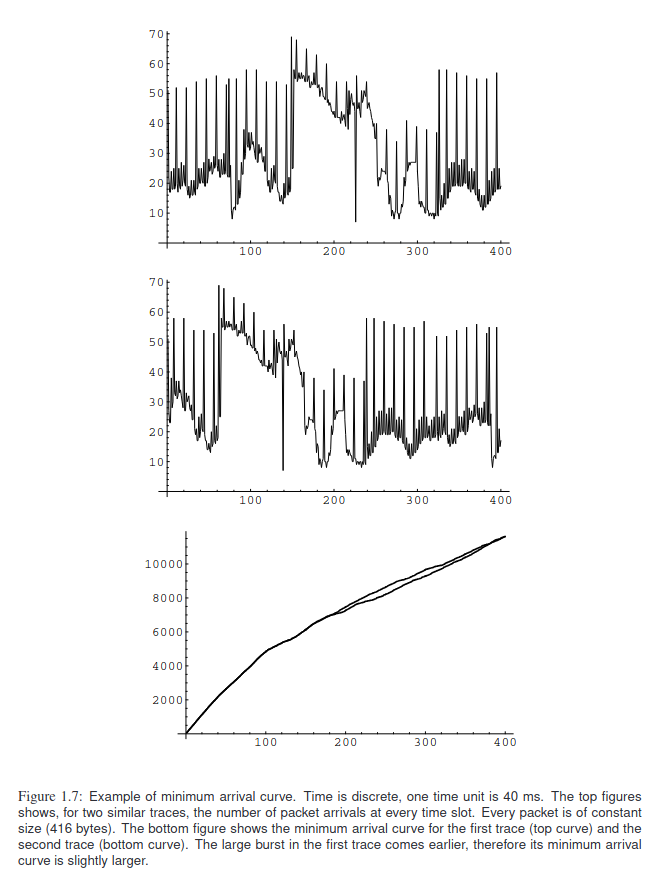
\includegraphics[width=.45\textwidth]{figs/min-arrival.png}
    \end{figure}
\end{frame}




\subsection{Curvas de servicio}
\begin{frame}{\secname: \subsecname}
    \begin{definition}[Curva de servicio]
        Sea un flujo $R$ atravesando
        un sistema $\mathcal{S}$,
        decimos que $\beta\in\mathcal{F}$
        es una curva de servicio
        de $R\in\mathcal{F}$ si y solo si
        \begin{equation*}
            R^*\geq R\otimes\beta
        \end{equation*}
    \end{definition}

    \vfill

    \begin{figure}[h]
        \centering
        \begin{tikzpicture}[
  declare function={
    ratelatency(\R,\T,\x)= (\x<=\T) * 0   +
    (\x>\T) * (\R*(\x-\T));
    },
  declare function={
    rateburst(\r,\b,\x)= (\x<=0) * 0   +
    (\x>0) * (\r*\x+\b);
    },
]
\begin{axis}[
    x=1cm,
    y=1cm,
    domain=0:5,
    ymin=0,
    ymax=3,
    xmin=0,
    xmax=4,
    axis x line=middle,
    axis y line=middle,
     xlabel style={
            anchor=west,
            at={(ticklabel* cs:1.0)},
            xshift=5pt
        },
     ylabel style={
            anchor=west,
            at={(ticklabel* cs:1.0)},
            xshift=.1pt
        },
    xlabel=$t$,
    ylabel={bits},
    legend pos=outer north east
    ]
    \addplot[Firebrick2,ultra thick]
        {5*log10(x+1)};

    \addplot[DodgerBlue2,ultra thick,
        samples=1000]
        {ratelatency(1,1,x)};

    \addplot[Firebrick4,ultra thick,domain=0.8:5]
        {4.9*log10(x+.2)};

    \addplot[DodgerBlue2,ultra thick,
        samples=1000]
        {ratelatency(1,1,x)};


    \foreach \t in {0.5,1,1.5,2} {
    \addplot[DodgerBlue4,thick,
        samples=1000,domain=\t:5]
        {ratelatency(1,1,x-\t)+5*log10(\t+1)};
        
    }
    

    \legend{$R(t)$,$\beta(t)$,$R^*(t)$};


    % \addplot[Firebrick3,ultra thick,samples=1000]
    %     {3*log10(x+1)};

    %\addplot[Gold3,ultra thick,smooth,samples=1000]
    %    {(x>=-1.3)*(0.3*(\x+1.3)+1.1)+and(x>-2.6,x<-1.3)*(1.1+0.9*\x+0.9*1.3)};



    % \legend{$R^*(t)$,
    % $R(t)$
    % ,$(f\oslash g)(t)$
    % };

   % \node (burstop) at (axis cs:0.1,1.2){};
   % \node (burstbottom) at (axis cs:0.1,-.1){};
   % \draw[|-|](burstop)--(burstbottom)
   %     node[midway,right]
   %     {$b$};


   %\draw[|-|, gray]
   %    (axis cs:.15,.2)
   %    --
   %    (axis cs:1.3,.2)
   %    node[pos=.9,above]
   %    {$T$};



\end{axis}
\end{tikzpicture}

    \end{figure}
\end{frame}



\begin{frame}{\secname: \subsecname}
    La curva de servicio ``rate-latency''
    es $\beta_{R,T}(t)=R[t-T]^+$.

    \vfill

    La curva de servicio
    ``burst-delay'' es
    \begin{equation*}
        \delta_T(t)=\begin{cases}
            +\infty,\quad t>T\\
            0, \quad t\leq T
        \end{cases}
    \end{equation*}

    \vfill
    
    \begin{figure}[h]
        \centering
        \begin{tikzpicture}[
  declare function={
    ratelatency(\R,\T,\x)= (\x<=\T) * 0   +
    (\x>\T) * (\R*(\x-\T));
    },
  declare function={
    rateburst(\r,\b,\x)= (\x<=0) * 0   +
    (\x>0) * (\r*\x+\b);
    },
]
\begin{axis}[
    x=1cm,
    y=1cm,
    domain=0:5,
    ymin=0,
    ymax=3,
    xmin=0,
    xmax=4,
    axis x line=middle,
    axis y line=middle,
     xlabel style={
            anchor=west,
            at={(ticklabel* cs:1.0)},
            xshift=5pt
        },
     ylabel style={
            anchor=west,
            at={(ticklabel* cs:1.0)},
            xshift=.1pt
        },
    xlabel=$t$,
    ylabel={bits},
    legend pos=outer north east
    ]
    \addplot[Firebrick3,ultra thick]
        {(x<2)*0+(x>=2)*100 + .05};

    \addplot[DodgerBlue3,ultra thick,
        samples=1000]
        {ratelatency(1,2,x)};

    

    \legend{$\delta_T(t)$,$\beta_{R,T}(t)$};


    % \addplot[Firebrick3,ultra thick,samples=1000]
    %     {3*log10(x+1)};

    %\addplot[Gold3,ultra thick,smooth,samples=1000]
    %    {(x>=-1.3)*(0.3*(\x+1.3)+1.1)+and(x>-2.6,x<-1.3)*(1.1+0.9*\x+0.9*1.3)};



    % \legend{$R^*(t)$,
    % $R(t)$
    % ,$(f\oslash g)(t)$
    % };

   % \node (burstop) at (axis cs:0.1,1.2){};
   % \node (burstbottom) at (axis cs:0.1,-.1){};
   % \draw[|-|](burstop)--(burstbottom)
   %     node[midway,right]
   %     {$b$};


   %\draw[|-|, gray]
   %    (axis cs:.15,.2)
   %    --
   %    (axis cs:1.3,.2)
   %    node[pos=.9,above]
   %    {$T$};



\end{axis}
\end{tikzpicture}

    \end{figure}
\end{frame}


\subsection{Concatenación}
\begin{frame}{\secname: \subsecname}
    Si atravesamos $N$ sistemas, cada
    uno con una curva de servicio
    $\beta_i,i=1,\ldots,N$; la curva
    de servicio del sistema total
    es
    \begin{equation*}
        \beta
        =\beta_1\otimes\beta_2
        \ldots\otimes\beta_N
        =\otimes_{i=1}^N\beta_i
    \end{equation*}

    \vfill

    \begin{figure}[h]
        \centering
        \begin{tikzpicture}
    \node[circle,draw]
        (system)
        at (0,0) {$\mathcal{S}_1$};

    \node[circle,draw]
        (system2)
        at (1,0) {$\mathcal{S}_2$};

    \node
        (systemdots)
        at (2,0) {$\ldots$};

    \node[circle,draw]
        (systemN)
        at (3,0) {$\mathcal{S}_N$};


    \draw[->,ultra thick,Firebrick2]
        ($(system)-(2,0)$)
        node[left]
        {$R$}
        --
        (system.west)
        ;

    \draw[->,ultra thick,DodgerBlue2]
        (systemN.east)
        --
        ($(systemN)+(2,0)$)
        node[right]
        {$R^*$}
        ;

    
\end{tikzpicture}

    \end{figure}
\end{frame}



\begin{frame}{\secname: \subsecname}
    \emph{Ejemplo}: concatenación
    de curvas rate-latency.

    \begin{equation*}
        (\beta_{R_1,T_1}\otimes
        \beta_{R_2,T_2})
        =\beta_{\min\{R_1,R_2\},T_1+T_2}
    \end{equation*}


    \begin{figure}[h]
        \centering
        \begin{tikzpicture}[
  declare function={
    ratelatency(\R,\T,\x)= (\x<=\T) * 0   +
    (\x>\T) * (\R*(\x-\T));
    }
]
\begin{axis}[
    x=0.5cm,
    y=1cm,
    domain=0:5,
    ymin=0,
    xmin=0,
    axis x line=middle,
    axis y line=middle,
     xlabel style={
            anchor=west,
            at={(ticklabel* cs:1.0)},
            xshift=5pt
        },
        xlabel=$t$,
    ]
    \addplot[DodgerBlue3,ultra thick,smooth]
        {ratelatency(0.5,1,x)};
    \node[DodgerBlue3] at (axis cs:1.5,1)
        {$\beta_{R_1,T_1}$};
\end{axis}
\end{tikzpicture}
\begin{tikzpicture}[
  declare function={
    ratelatency(\R,\T,\x)= (\x<=\T) * 0   +
    (\x>\T) * (\R*(\x-\T));
    }
]
\begin{axis}[
    x=0.5cm,
    y=1cm,
    domain=0:5,
    ymin=0,
    ymax=2,
    xmin=0,
    xmax=4,
    axis x line=middle,
    axis y line=middle,
     xlabel style={
            anchor=west,
            at={(ticklabel* cs:1.0)},
            xshift=5pt
        },
        xlabel=$t$,
    ]
    \addplot[Firebrick3,ultra thick,smooth]
        {ratelatency(1,2,x)};
    \node[Firebrick3] at (axis cs:1.5,1)
        {$\beta_{R_2,T_2}$};
\end{axis}
\end{tikzpicture}
\begin{tikzpicture}[
  declare function={
    ratelatency(\R,\T,\x)= (\x<=\T) * 0   +
    (\x>\T) * (\R*(\x-\T));
    }
]
\begin{axis}[
    x=0.5cm,
    y=1cm,
    domain=0:5,
    ymin=0,
    ymax=2,
    xmin=0,
    axis x line=middle,
    axis y line=middle,
     xlabel style={
            anchor=west,
            at={(ticklabel* cs:1.0)},
            xshift=5pt
        },
        xlabel=$t$,
    ]
    \addplot[Gold3,ultra thick,smooth]
        {ratelatency(0.5,3,x)};
    \node[Gold4] at (axis cs:2,1)
        {$\otimes_i\beta_i$};
\end{axis}
\end{tikzpicture}

    \end{figure}
\end{frame}




\section{Resultados fundamentales}
\subsection{Retardo y backlog}
\begin{frame}{\secname: \subsecname}
    \begin{definicion}[Retardo y backlog]
        Sea un flujo $R\in\mathcal{F}$
        que al atravesar
        el sistema $\mathcal{S}$
        sale como $R^*\in\mathcal{F}$,
        el retardo de un bit que
        llega en $t$ se define como
        \begin{equation*}
            d(t)=\inf_{\tau>0}
            \{\tau: R(t)\leq R^*(t+\tau)\}
        \end{equation*}
        y el backlog en el instante $t$
        como
        \begin{equation*}
            x(t)=R(t)-R^*(t)
        \end{equation*}
    \end{definicion}

    \begin{figure}[h]
        \centering
        \begin{tikzpicture}[
  declare function={
    ratelatency(\R,\T,\x)= (\x<=\T) * 0   +
    (\x>\T) * (\R*(\x-\T));
    },
  declare function={
    rateburst(\r,\b,\x)= (\x<=0) * 0   +
    (\x>0) * (\r*\x+\b);
    },
]
\begin{axis}[
    x=1.5cm,
    y=.9cm,
    domain=0:5,
    ymin=0,
    ymax=2,
    xmin=0,
    xmax=3,
    axis x line=middle,
    axis y line=middle,
     xlabel style={
            anchor=west,
            at={(ticklabel* cs:1.0)},
            xshift=5pt
        },
     ylabel style={
            anchor=west,
            at={(ticklabel* cs:1.0)},
            xshift=.1pt
        },
    xlabel=$t$,
    ylabel={bits},
    legend pos=outer north east
    ]
    \addplot[Firebrick3,ultra thick]
        {5*log10(x+1)};


    \addplot[DodgerBlue3,ultra thick,domain=0.8:5]
        {4.9*log10(x+.2)};



    \legend{$R(t)$,$R^*(t)$};


    % \addplot[Firebrick3,ultra thick,samples=1000]
    %     {3*log10(x+1)};

    %\addplot[Gold3,ultra thick,smooth,samples=1000]
    %    {(x>=-1.3)*(0.3*(\x+1.3)+1.1)+and(x>-2.6,x<-1.3)*(1.1+0.9*\x+0.9*1.3)};



    % \legend{$R^*(t)$,
    % $R(t)$
    % ,$(f\oslash g)(t)$
    % };

   % \node (burstop) at (axis cs:0.1,1.2){};
   % \node (burstbottom) at (axis cs:0.1,-.1){};
   % \draw[|-|](burstop)--(burstbottom)
   %     node[midway,right]
   %     {$b$};


   %\draw[|-|, gray]
   %    (axis cs:.15,.2)
   %    --
   %    (axis cs:1.3,.2)
   %    node[pos=.9,above]
   %    {$T$};


    \draw[|-|]
        (axis cs:0,.1)
        --
        (axis cs:.8,.1)
        node[pos=.8,above]
        {$d(0)$};

    \draw[|-|]
        (axis cs:1,.5)
        --
        (axis cs:1,1.4)
        node[pos=.7,right,rotate=20]
        {$x(1)$};


\end{axis}
\end{tikzpicture}

    \end{figure}

\end{frame}



\subsection{Cotas retardo/backlog}
\begin{frame}{\secname: \subsecname}
    \begin{lema}[Cota retardo/backlog]
        Sea un flujo $R\in\mathcal{F}$
        con curva de llegada
        $\alpha$ que atraviesa un
        sistema $\mathcal{S}$ con
        curva de servicio $\beta$,
        el retardo y backlog cumplen
        \begin{align*}
            d(t)&\leq h(\alpha,\beta)\\
            x(t)&\leq v(\alpha,\beta)
        \end{align*}
    \end{lema}
\end{frame}


\begin{frame}{\secname: \subsecname}
    \emph{Ejemplo}: si tenemos 
    las curvas $\alpha=\gamma_{r,b}$
    y $\beta_{R,T}$, las cotas de
    retardo y backlog son
    \begin{align*}
        d(t)\leq \frac{b}{R}+T\\
        x(t)\leq rT+b
    \end{align*}
    \begin{figure}[h]
        \centering
        \begin{tikzpicture}[
  declare function={
    ratelatency(\R,\T,\x)= (\x<=\T) * 0   +
    (\x>\T) * (\R*(\x-\T));
    }
]
\begin{axis}[
    x=1cm,
    y=1cm,
    domain=0:5,
    ymin=0,
    xmin=0,
    axis x line=middle,
    axis y line=middle,
     xlabel style={
            anchor=west,
            at={(ticklabel* cs:1.0)},
            xshift=5pt
        },
    xlabel=$t$,
    legend pos=outer north east
    ]
    \addplot[DodgerBlue3,ultra thick,smooth]
        {ratelatency(0.9,1.3,x)};
    \addplot[Firebrick3,ultra thick,samples=1000]
        {(x>0)*(0.3*\x+1.1) + (x<0)*0};

    %\addplot[Gold3,ultra thick,smooth,samples=1000]
    %    {(x>=-1.3)*(0.3*(\x+1.3)+1.1)+and(x>-2.6,x<-1.3)*(1.1+0.9*\x+0.9*1.3)};



    \legend{$\alpha_{r,b}(t)$,
    $\beta_{R,T}(t)$
    %,$(f\oslash g)(t)$
    };

   % \node (burstop) at (axis cs:0.1,1.2){};
   % \node (burstbottom) at (axis cs:0.1,-.1){};
   % \draw[|-|](burstop)--(burstbottom)
   %     node[midway,right]
   %     {$b$};

   \draw[<->,thick]
       (axis cs:0,1.1)
       --
       (axis cs:2.5,1.1)
       node[pos=.9,above]
       {\small $h(f,g)$};

   \draw[<->,thick,gray]
       (axis cs:1.3,0)
       --
       (axis cs:1.3,1.5)
       node[pos=.3,left]
       {\small $v(f,g)$};

   %\draw[|-|, gray]
   %    (axis cs:.15,.2)
   %    --
   %    (axis cs:1.3,.2)
   %    node[pos=.9,above]
   %    {$T$};

   % \draw[|-|, gray]
   %     (axis cs:-.05,.2)
   %     --
   %     (axis cs:-1.3,.2)
   %     node[midway,above]
   %     {$T$};


\end{axis}
\end{tikzpicture}

    \end{figure}
\end{frame}



\begin{frame}{\secname: \subsecname}
    \emph{Ejemplo (cont.)}: 
    recordemos la deconvolución 
    \begin{equation*}
        (\gamma_{r,b}
        \oslash
        \beta_{R,T})(t)
        =
        \begin{cases}
            [b+R(t+T)]^+,\quad t\leq -T\\
            r(t+T)+b,\quad t>-T
        \end{cases}
    \end{equation*}
    Recordemos también que la
    desviación horizontal se puede
    calcular como
    $h(\gamma_{r,b},\beta_{R,T})
    =\inf_{u\geq0}\{
        d: (\gamma_{r,b}\oslash\beta_{R,T})(-d)
    \leq0
    \}$.
    Buscamos dónde se hace cero la
    deconvolución:
    \begin{align*}
        t&=-(\frac{b}{r}+T),\quad t\leq -T\\
        t&=-(\frac{b}{R}+T),\quad t>-T
    \end{align*}

    Por tanto la desviación horizontal es
    $h(\gamma_{r,b},\beta_{R,T})
    =\frac{b}{R}+T$.

\end{frame}



\subsection{Prioridades}
\begin{frame}{\secname: \subsecname}
    \begin{lema}[Curvas de servicio
        sistema con prioridades]
        Sean dos flujos $R_L,R_H\in\mathcal{F}$
        con curvas de llegadas
        $\alpha_L,\alpha_H$
        que atraviesan un sistema
        $\mathcal{S}$ con curva de servicio
        $\beta$ que da prioridad
        a $R_H$, las curvas 
        de servicio que experimentan
        los flujos de alta/baja prioridad
        son
        \begin{align*}
            \beta_H=[\beta-l_{\max}^L]^+\\
            \beta_L=[\beta-\alpha_H]^+
        \end{align*}
        con $l_{\max}^L$ el tamaño máximo
        de paquete del flujo de baja
        prioridad.
    \end{lema}
\end{frame}



\begin{frame}{\secname: \subsecname}
    \emph{Ejemplo:} la cola de
    prioridad luego atraviesa
    un sistema con curva de servicio
    rate latency $\beta_{R,T}$.
    Además el flujo de prioridad
    $R_H$ es $\gamma_{r,b}$-suave.


    \vfill
    \begin{figure}[h]
        \centering
        \begin{tikzpicture}


    % queue H
    \draw
        (0,-1)
        --
        (1.5,-1)
        --
        (1.5,-1.5)
        --
        (0,-1.5);


    % queue H
    \draw
        (0,-2)
        --
        (1.5,-2)
        --
        (1.5,-2.5)
        --
        (0,-2.5);

    % H flow
    \draw[->,ultra thick,Firebrick4]
        (-1,-1.25)
        node[left]
        {$R_H$}
        --
        (0,-1.25);

    % L flow
    \draw[->,ultra thick,Firebrick2]
        (-1,-2.25)
        node[left]
        {$R_L$}
        --
        (0,-2.25);


    \node[draw,circle]
        (circle)
        at
        (2,-1.75)
        {$R$};

    \draw[->,ultra thick]
        (circle)
        --
        ($(circle)+(2,0)$)
        node[midway,above,Firebrick4]
        {$R^*_H$}
        node[midway,below,Firebrick2]
        {$R^*_L$}
        ;

    
    
\end{tikzpicture}

    \end{figure}
    \vfill

    En este caso se tiene
    \begin{align*}
        \beta_H=\beta_{R,\tfrac{l_{\max}^L}{R}}\\
        \beta_L=\beta_{R-r,\tfrac{b}{R-r}}
    \end{align*}


\end{frame}



\subsection{Weighted Fair Queuing}
\begin{frame}{\secname: \subsecname}
    En el caso del WQF cada flujo
    $i$ recibe un peso
    $w_i/\sum_{j\neq i}w_j$.
    Por tanto el flujo $R_i$ experimenta
    una curva de servicio
    \begin{equation*}
        \beta_{\frac{w_i}{\sum_{j\neq i}w_j},0}
    \end{equation*}
\end{frame}




\begin{frame}[allowframebreaks]
        \frametitle{Referencias}
        \bibliographystyle{amsalpha}
        \bibliography{refs.bib}
\end{frame}


\end{document}
